\documentclass[
	12pt
] {article}

\usepackage[
	a4paper,
	left=3cm,
	right=2cm,
	top=3cm,
	bottom=3cm
] {geometry} %for setting margin

\usepackage{parskip}
\usepackage{mathtools}
\usepackage{authblk} %authors and their affiliations
\usepackage{graphicx} %for include graphics
\graphicspath{{figures/}}

\title{Two-phase imbibition in Porous Media using a Two-dimensional Network Model}

\author[1, 2]{Kafi Shabbir}
\author[1, 3]{Oleg Izvekov}
\author[1, 4]{Andrey Konyukhov}
\affil[1]{Moscow Institute of Physics and Technology, Dolgoprudny, 141701}
\affil[2]{kafiulshabbir@phystech.edu}
\affil[3]{izvekov\_o@inbox.ru}
\affil[4]{konyukhov\_av@mail.ru}

\begin{document}
\nocite{*}
\maketitle
UDK: 532.685

\begin{abstract}
	 This article is about a 2D network model, which we developed for simulating imbibition of two-phase flow in porous media. Our 2D plane of porous media consisted of two regions: the outer region with thicker tubes was initially saturated with wetting fluid, and the inner region with thinner tubes with non-wetting fluid. We measured the saturation of wetting fluid $S$  with respect to time $t$, and the average capillary pressure $P_c$ with respect to $S$ in the inner region. Our network model used a novel method of distributing fluids at the nodes, which is when more than two phases enter a node at the same time, the wetting fluid is distributed first according to the ascending order of the radii of the tubes. Simulation results showed that the wetting fluid indeed invaded the inner region and displaced the non-wetting fluid to the outer region, and the plots of $S(t)$ and $P_c(S)$ qualitatively matches other references. Therefore, the novel method of distributing different phases at nodes and our network model is valid in general.
\end{abstract}

\textbf{Keywords:} imbibition, capillary pressure, non-equilibrium effect, phase distribution

This project was supported by Russian Science Foundation, grant 23-21-00175.

\section{Introduction} \label{sec:intro}
	Modeling and simulation of two-phase flow in porous media is important due many applications in oil recovery, hydrology, electricity production, etc \cite{labed2012experimental}. Porous media consists of a skeletal material (usually solid) and voids (also called pores). The voids are connected to each other by other narrow tube like voids called capillaries. The voids are usually filled with fluids such as water, oil or gases \cite{su2012insights}. Saturation of a fluid $S_i$ is defined as the ratio between the volume $V_{i}$ occupied by ${fluid}_i$ to the total volume of the void $V_{void}$:
	
	\begin{equation}
		S_{i} = \frac{V_{i}}{V_{void}}
	\end{equation}
	
	Since we consider only two fluids: wetting of saturation $S_w$ such as water, and non wetting of saturation $S_{nw}$ such as oil in the voids. The two quantities are related by: $S_{w} + S_{nw} = 1$. For simplicity, let $S$ denote the saturation of the wetting fluid. Classical continuum models, such as Darcy's Law \cite{darcy1856fontaines} are still commonly used:
	\begin{equation}
		q = -\frac{k}{\mu} \nabla P
	\end{equation}
	
	Here, $q$ is the flow rate, $k$ is the permeability, $\mu$ is the coefficient of viscosity, and $\nabla P$ is the pressure gradient.
	
	In classical continuum models, the permeability is only a function of the saturation of one of the fluid $k = k(S)$ [REF?].
	
	The classical continuum models are valid as long as the characteristic time of the processes is much longer than the characteristic time of fluid redistribution in the capillary space. The fluid distribution can take longer time due to non-equilibrium effects, which occurs when the saturation changes rapidly, or the porous medium is a fractured with blocks and cracks [REF?]. In these cases, the assumption that permeability is only a function of the saturation is not sufficient, and additional parameters are required. Various advanced continuum models \cite{hassanizadeh2004continuum}, \cite{hassanizadeh1987high}, \cite{barenblatt1960basic} consider such non-equilibrium effects, by assuming the permeability $k$ to additionally be a function of the rate of change of saturation with respect to time:
	
	\begin{equation} \label{eq:conn-adv-model-perm}
		k = k(S, \frac{\partial S}{\partial t})
	\end{equation}

	[COMMENT: Why is the Kondaurov model, better? Or in which situation is it more useful than advanced continuum models described by equation \ref{eq:conn-adv-model-perm}]. The Kondaurov model \cite{kondaurov2009non} considers a special non-equilibrium parameter $\xi$ along with saturation $S$, which relaxes to an equilibrium value \cite{kondaurov2007thermodynamically}.
	
	\begin{equation}
		k = k(S, \xi)
	\end{equation}
	
	And $\xi$ is related to $S$ by the differential equation [COMMENT: by "a" or by "the" differential equation?]:
	
	\begin{equation}
		\frac{\partial \xi}{\partial t} = \Omega ( S, \xi )
	\end{equation}
		
	Here, $\Omega$ is an arbitrary function [COMMENT: verification needed].
	
	In order to better understand the non-equilibrium characteristics, it is necessary to develop non-continuum models and simulate the flow at the scale of pores. Some of the methods of modeling at the scale of pores are: Lattice Boltzmann Method [REF?], a direct Navier-Stokes simulation, or a network model [REF?, Citation about article which speaks about the various methods used to model non-continuum characteristics of porous media]. Direct Navier-Stokes simulation gives us very accurate results on velocity and pressure distributions, but it is very complicated [REF?, add citation]. Network models are much simpler. Our aim is to develop a network model which will help better understand non-equilibrium characteristics of two-phase flow, and observe the Kondaurov's non-equilibrium parameter resting at an equilibrium value.
	
\section{Theory}
\subsection{Characteristics of our network model}
	\begin{figure}
		\centering
		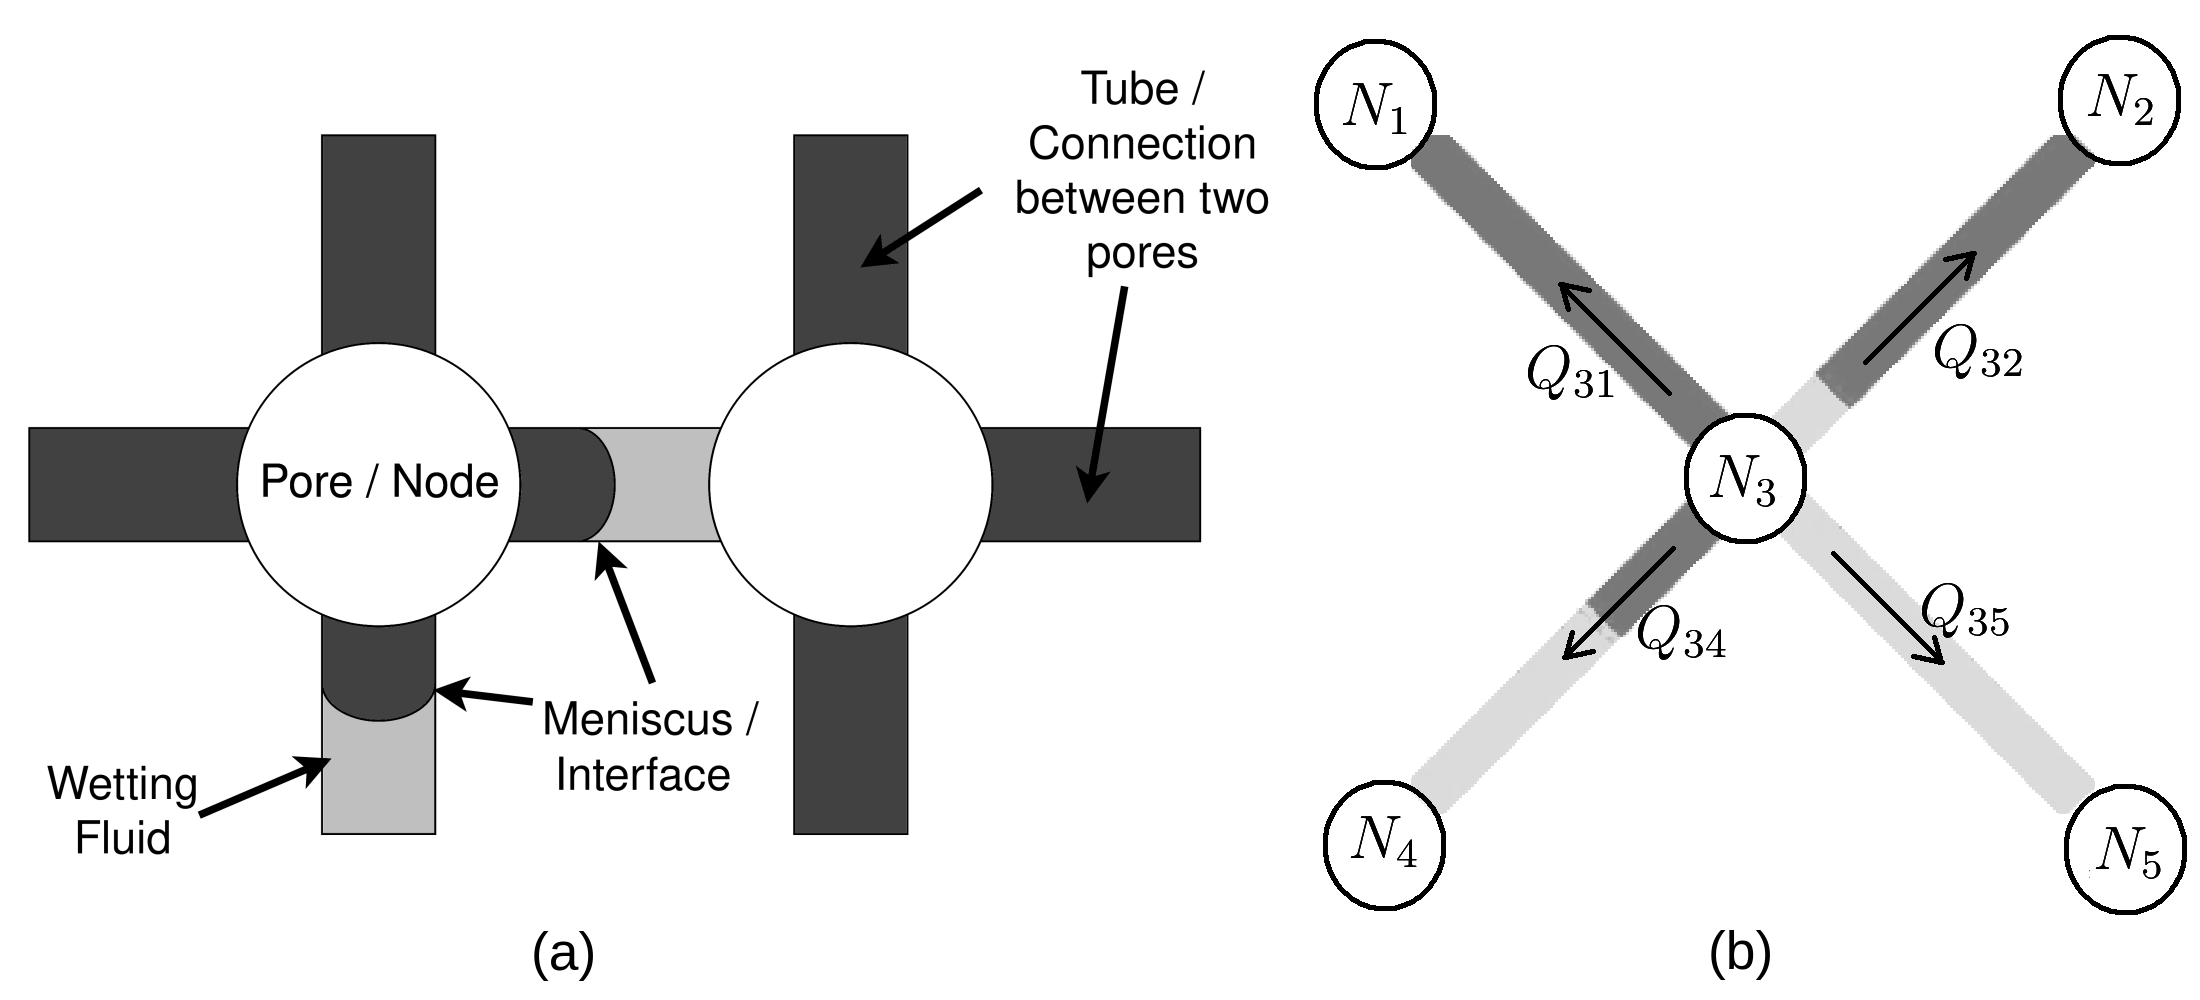
\includegraphics[width=\textwidth]{fig_1_2200x1000}
		\caption{Network model as an approximation of porous media (a), with pores as nodes, and capillaries as tubes. Flow rates $Q$ out of Node $N_3$ (b).}
		\label{fig:1}
	\end{figure}
	
	In our network model, the pores are represented by nodes, and capillaries by tubes, as shown in figure \ref{fig:1}a. Our model is two-dimensional (2D), and each node is connected to 4 other nodes by tubes of the same length, as also shown in figure \ref{fig:1}b, and is similar to \cite{aker1998two}. They considered tubes to be hour glass shaped and used approximate flow rate equations \cite{washburn1921dynamics}, however we used only cylindrical tubes, because it allowed us to derive and use exact flow rate equations. In our model, the tubes can have different radii, and a maximum of 2 menisci.
	
	A node may be connected to less than 4 nodes, when they are located at the boundaries, see figure \ref{fig:3}. The fluids are not compressible. The darker color always denotes non-wetting fluid, while the lighter color denotes wetting fluid. Gravity is ignored. The volume of the node is not taken into consideration and is assumed to be zero.
	
	\begin{figure}
		\centering
		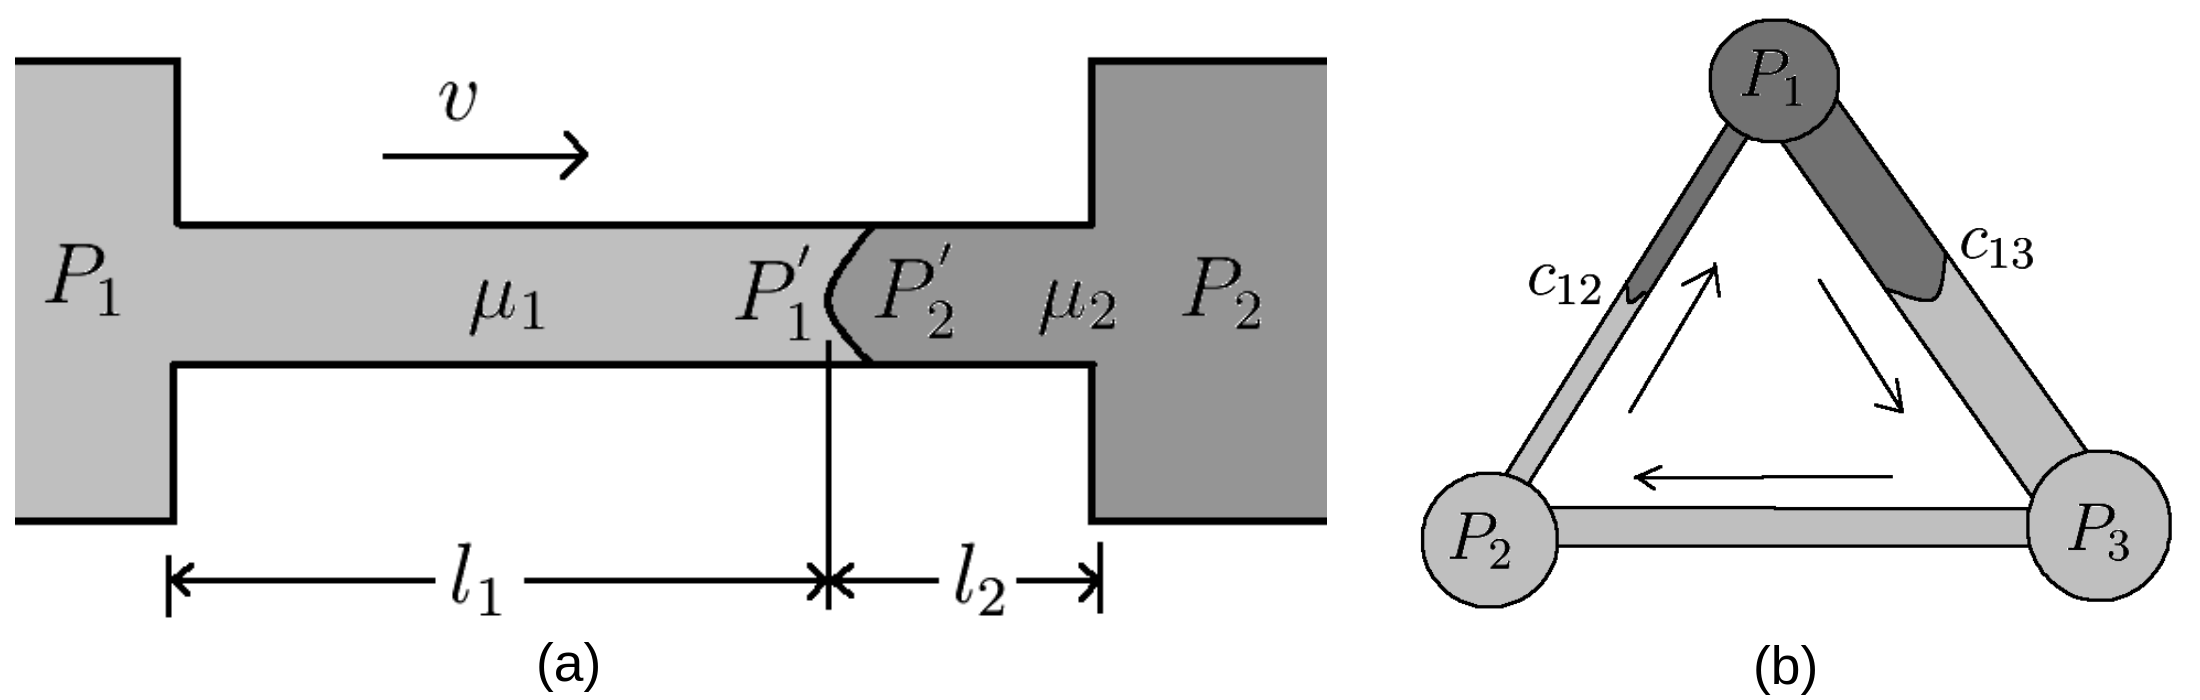
\includegraphics[width=\textwidth]{fig_2_2200x700}
		\caption{Flow in a tube with a meniscus and fluids of viscosity $\mu$,  (a). A simple example of a system with menisci and closed boundaries (b), where the pressure matrix has infinitely many solutions.}
		\label{fig:2}
	\end{figure}
	
\subsection{Average capillary pressure}
	The capillary pressure $p'$ is:
	\begin{equation}
		p' = \frac{2 \sigma}{R}
	\end{equation}
	
	Here, $\sigma$ is the coefficient of surface tension in $[Pa.m]$ or $[kg/s]$, $R$ is the radius of the tube.
	
	Let us define an function $Z$ dependent on the number of meniscus $n_{mns}$:
	\begin{equation} \label{eq:average-capillary-pressure-sign}
		Z(n_{mns}) = 
		\begin{dcases}
			0,&\text{$n_{mns}$ = 0, 2}\\
			1,&\text{$n_{mns}$ = 1}\\
		\end{dcases}
	\end{equation}
	
	We define the average capillary pressure $P_c$ in a region as:
	\begin{equation} \label{eq:average-capillary-pressure}
		P_c = \frac{\sum p'_i Z_i \pi R_i^2}{\sum Z_i \pi R_i^2}
	\end{equation}
	
\subsection{Flow rate in a tube with meniscus}
	The pressure jump across a meniscus for the tube in figure \ref{fid:2}a:
	\begin{equation} \label{eq:pressure-jump-def} 
		 p' = P_{2}' - P_{1}'
	\end{equation}
	
	We define the average viscosity parameter $M$, for a tube with multiple fluids of different viscosity $\mu$:
	\begin{equation} \label{eq:def-average-viscosity}
		M = \sum_{i} \mu_{i} \frac{l_{i}}{l}
	\end{equation}
	
	Here, $\mu$ is in $[kg/m.s]$, $l$ is the length of the tube.
	
	If $P_1 > P_2$ and the meniscus points towards $N_1$, then both pressure difference in the nodes and capillary pressure wants to move the fluid from $N_1$ to $N_2$, we
	\begin{enumerate}
		\item Write Hagen–Poiseuille equation \cite{sutera1993history} for parts of tubes of with same viscosity separately. For example, in figure \ref{fig:2}a: $Q(\mu_1 l_1) = A' (P_1 - P'_1)$ and $Q(\mu_2 l_2) = A' (P'_2 - P_2)$, here $A' = \pi R^4 / 8$
		\item Sum the equations.
		\item Replace the pressure jump $P'_2 - P'_1$ according to equation \ref{eq:pressure-jump-def}, and average viscosity parameter $M$ according to equation \ref{eq:def-average-viscosity}.
	\end{enumerate}
	And obtain:
	\begin{equation} \label{eq:flow-rate-main}
		Q = \frac{\pi R^4}{8Ml} \left( \Delta P_{12} + \frac{2 \sigma}{R} \right)
	\end{equation}
	
	Let us consider flow from an arbitrary Node $N_i$ to Node $N_j$, and $X_{ij}$ is the quantity associated with the tube connecting $N_i$ to $N_j$. We define $s$ to be a function which can only take the values of: $-1, 0, +1$, according to the orientation and the number of menisci present in the tube:
	
	\begin{equation}
		s_{ij}(d, n_{mns}) = 
		\begin{dcases}
			-1,&\text{$n_{mns}$ = 1, $d$ points away from $N_{i}$}\\
			0,&\text{$n_{mns}$ = 0, 2}\\
			+1,&\text{$n_{mns}$ = 1, $d$ points towards $N_{i}$}
		\end{dcases}
	\end{equation}

	Here, $d$ is the direction the convex side of the meniscus points towards. $n_{mns}$ is the number of meniscus in a tube.
	
	The flow rate equation of any $n_{mns}$:
	
	\begin{equation} \label{eq:flow-rate-simple}
		Q_{ij} = A_{ij}\Delta P_{ij} + B_{ij}
	\end{equation}
	
	Here, $\Delta P_{ij} = P_i - P_j$, and:
	\begin{equation} \label{eq:flow-rate-aij}
		A_{ij} = \frac{\pi R_{ij}^4}{8M_{ij}l}
	\end{equation}
	
	\begin{equation} \label{eq:flow-rate-bij}
		B_{ij} = \frac{\pi R_{ij}^4}{8M_{ij}l} \frac{2 s_{ij} \sigma}{R_{ij}}
	\end{equation}
	
	
	Since $M_{ij} = M_{ji}$ and $s_{ij} = -s_{ji}$, we have:
	\begin{equation}
		A_{ij} = A_{ji}
	\end{equation}
	\begin{equation}
		B_{ij} = -B_{ji}
	\end{equation}
	
	The flow velocity is:
	\begin{equation} \label{eq:vel-from-flow-rate}
		v_{ij} = \frac{ Q_{ij} }{\pi R_{ij}^2}
	\end{equation}
	
\subsection{Open system: filtration}
	In an open system, we can externally supply or remove fluid from the system. A simple example of an open system is filtration. For example, we have a block of porous media saturated with water. On the front face we apply high pressure of air, and keep the back face at a lower pressure. The air invades the porous block from the front face, and water leaves the porous block from the back face. 
	
	Figure \ref{fig:1}b is a very simple case of filtration. Here $N_4$ and $N_5$ are open and maintained at a constant higher pressure, while $N_1$ and $N_2$ are maintained at a constant lower pressure. We need to calculate the velocity at which the menisci will displace in each tube. The steps are:
	
	\begin{enumerate}
		\item We write a set linear equations to find the pressures in the nodes where it is not known.\item Since we know the pressures in all nodes, we can use equation \ref{eq:flow-rate-simple}, to determine the flow rates in each tube.
		\item The velocity at which the menisci will displace can now be calculated using equation \ref{eq:vel-from-flow-rate}.
	\end{enumerate}
		
	Let us look at how the linear equations are generated for filtration. Since the fluids are not compressible, the sum of volumetric flow out of $N_3$ is zero, or Kirchhoff's law is satisfied in figure \ref{fig:1}b:
	
	\begin{equation} \label{eq:sum-flow-node-zero}
		\sum_{k} Q_{3k} = 0
	\end{equation}
	
	Here, $k = {1, 2, 4, 5}$. We perform this sum in each of the nodes where the pressure is not known, and obtain a row for our pressure matrix:
	
	\begin{equation} \label{eq:matrix-open-sys-5-nodes}
		\begin{pmatrix}
			1 & 0 & 0 & 0 & 0 & P_{1}\\
			0 & 1 & 0 & 0 & 0 & P_{2}\\
			-A_{31} & -A_{32} & (A_{31} + ... + A_{35}) & -A_{34} & -A_{35} & -(B_{31} + ... + B_{35})\\
			0 & 0 & 0 & 1 & 0 & P_{4}\\
			0 & 0 & 0 & 0 & 1 & P_{5}
		\end{pmatrix}
	\end{equation}
	
	Here each column corresponds to coefficient in front of the variables: $P_1, P_2, ... P_5$.
	
	After solving the set of linear equations, we obtain the pressure at $N_3$. And once pressures at all nodes are known, we can calculate flow rates and velocities in all tubes.
	
\subsection{Closed system}	
	It can be proven that, we can take a network model of an arbitrary large size, and if we maintain high pressure at the bottom row of nodes, and low pressure on top row, the linear equations produce an unique solution and it is possible to determine the flow rates in all tubes. We have simulated the process of filtration and verified that our model works. However, in order to simulate imbibition, we need a closed system. Figure \ref{fig:2}b is a simple example of a closed system, whose pressure matrix can be written as:
	
	\begin{equation}
		\begin{pmatrix}
			(A_{12} + A_{13}) & -A_{12} & -A_{13} & -B_{12} - B_{13} \\
			-A_{21} & (A_{21} + A_{23}) & -A_{23} & -B_{21} - B_{23} \\
			-A_{31} & -A_{32} & (A_{31} + A_{32}) & -B_{31} - B_{32} \\
		\end{pmatrix}
	\end{equation}
	
	Since $B_{ij} = - B_{ji}$, we see that the sum of each column in this matrix is zero. Therefore, there are infinitely many solutions. We have solved this problem by, adding a non zero constant $a$ to the 3rd column.
	
	\begin{equation}
		\begin{pmatrix}
			(A_{12} + A_{13}) & -A_{12} & -A_{13} + a & -B_{12} - B_{13} \\
			-A_{21} & (A_{21} + A_{23}) & -A_{23} + a & -B_{21} - B_{23} \\
			-A_{31} & -A_{32} & (A_{31} + A_{32}) + a & -B_{31} - B_{32} \\
		\end{pmatrix}
	\end{equation}
	
	Then the sum of all columns give us $3aP_3 = 0$, which means $P_3 = 0$. It can be shown that any node in the system can be assumed to have zero pressure, the pressure difference which determines the flow rate is not affected by the choice of node where we assume zero pressure. 

\subsection{Fluid distribution in nodes (novel method)} \label
	There are situations when both wetting and non-wetting fluid enters a node. According to our novel method, we insert the wetting fluid first into tubes in ascending order of their radius.
	
	For example, we have solved the set of linear equations and chosen an appropriate time step to integrate, we know the volume of each fluid that will enter the node and will leave the node, their sum must be equal due to the conservation of volume. ${tube}_1$ is thinner than ${tube}_4$. Now let us look at certain cases:
	\begin{enumerate}
		\item $0.6 u$ (unit volumes) of wetting fluid, and $0.4 u$ of non-wetting fluid enters a node from ${tube}_1$ and ${tube}_2$, it does not matter how much of wetting fluid came from which tube. And from calculated flow rates, we know that $0.2 u$ must flow into ${tube}_3$ and $0.8 u$ must flow into $tube_4$:
		
		\begin{enumerate}
			\item $0.2 u$ of wetting fluid in inserted into ${tube}_3$.
			\item $0.6 - 0.2 = 0.4 u$ of wetting fluid is first inserted into ${tube}_4$.
			\item Then $0.4 u$ of non-wetting fluid is inserted into ${tube}_4$.
		\end{enumerate}
		
		\item  $0.6 u$ (unit volumes) of wetting fluid, and $0.4 u$ of non-wetting fluid enters a node from ${tube}_1$ and ${tube}_2$, it does not matter how much of wetting fluid came from which tube. And from calculated flow rates, we know that $0.2 u$ must flow into ${tube}_3$ and $0.8 u$ must flow into $tube_4$:
	\end{enumerate}


\section{Experiment}
	\begin{figure}
		\centering
		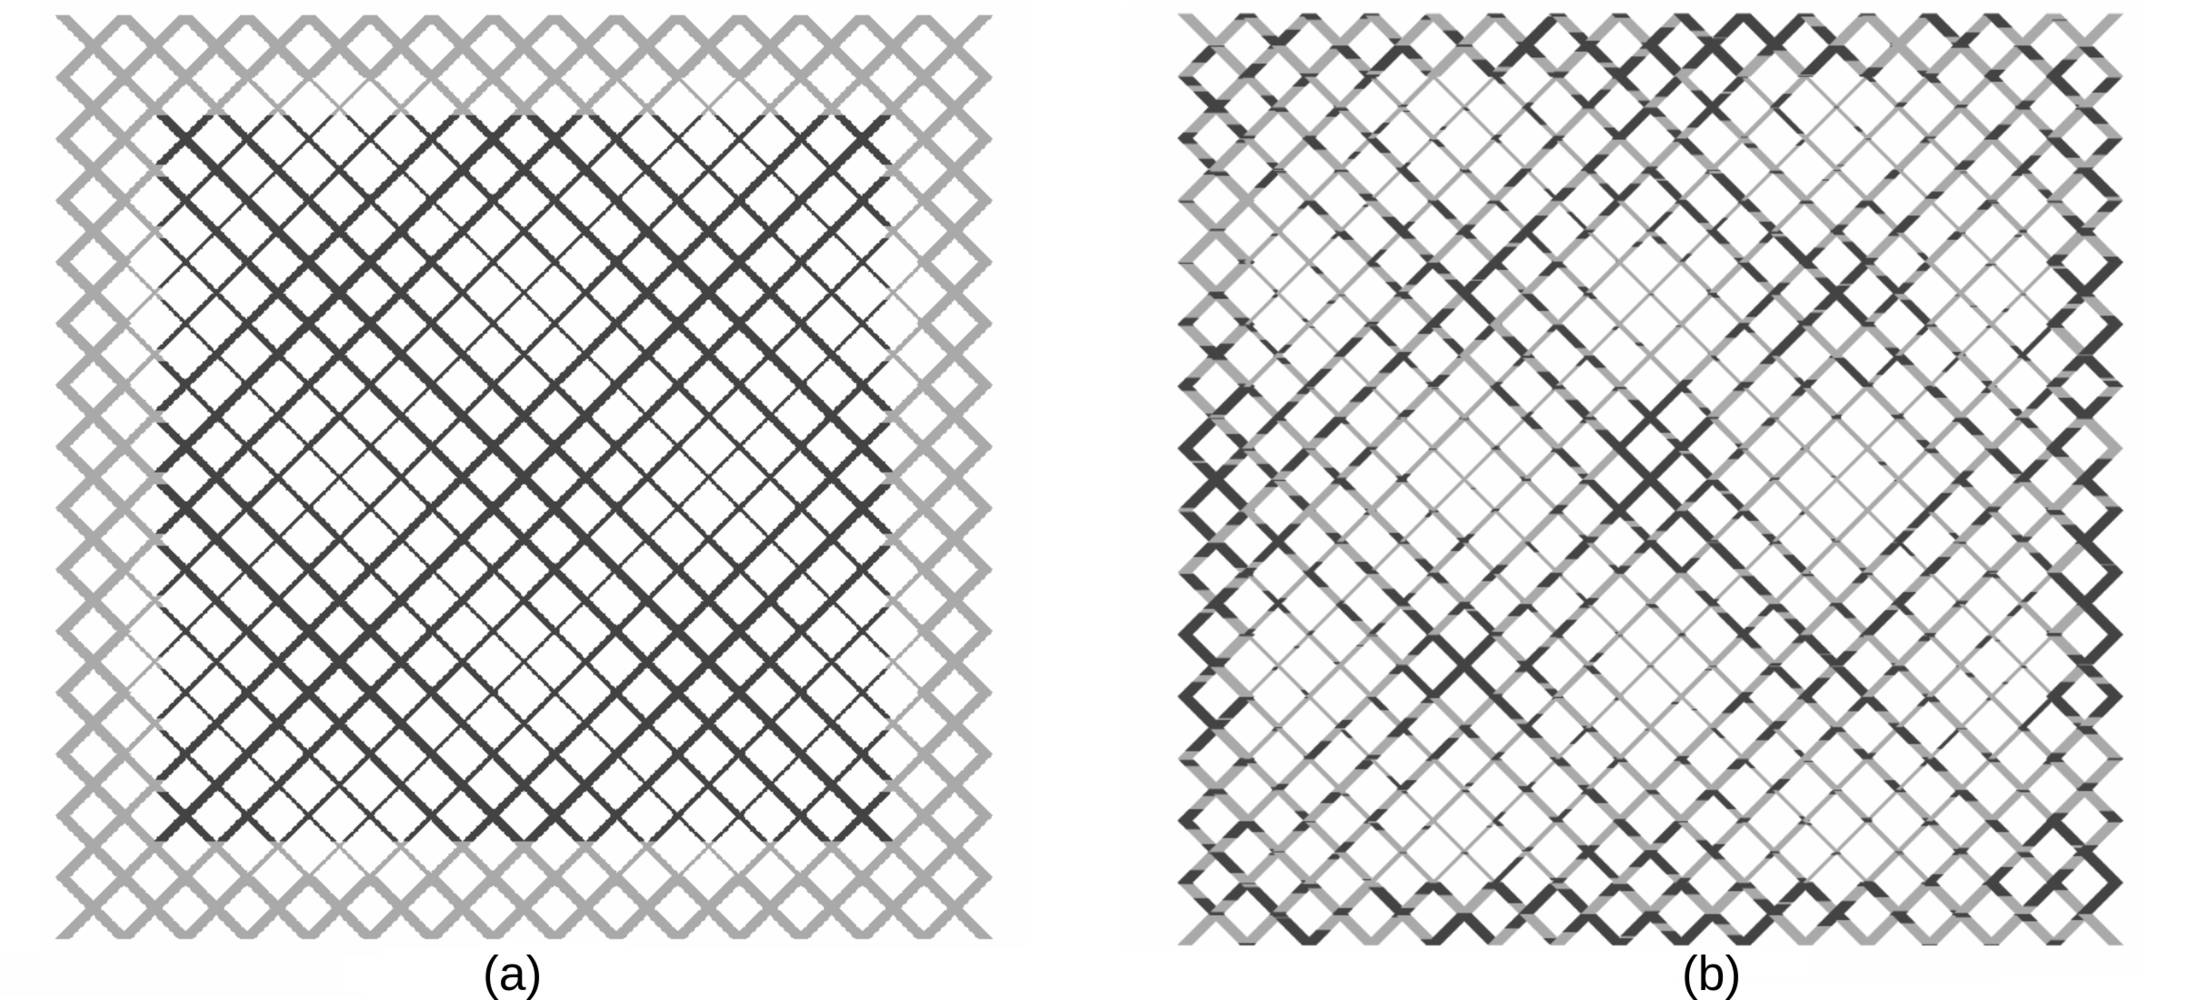
\includegraphics[width=\textwidth]{fig_3_2200x1000}
		\caption{Wetting fluid (lighter color) initially situated in the outer region with thicker tubes, non-wetting fluid (darker color) in the inner region saturated with thicker tubes (a). After simulation and we see that non-wetting fluid (dark) mostly occupies the intersection of the thicker tubes, and wetting fluid (b) occupies the thinner tubes.}
		\label{fig:3}
	\end{figure}

\subsection{Initial location of wetting and non-wetting fluid}
	In simulation of imbibition, wetting fluid was situated in the outer region, and non-wetting fluid in the inner region as shown in figure \ref{fig:3}. It is clear that the capillary pressure at the corners are greater. Therefore the wetting fluid invades the inner region from the corners of the inner region and displaces the non-wetting fluid from the edges.
	
\subsection{Radius distribution of tubes}
	The two rows along the perimeter have thicker radius of $6 m$ and inner region radii of range $(2, 3, ..., 5) m$, capillaries in nature cannot be so thick, we are only interested in the qualitative shape of the plots, so we have used dimensionless time. The volume of the inner region is approximately equal to the volume of the outer region.
	
\subsection{Measurement goals}
\begin{enumerate}
	\item To measure the saturation of wetting fluid $S(t)$ with respect to time, and check if it reaches an equilibrium value according to Kondaurov [?REF].
	\item To calculate the final average capillary pressure $P_c$ for the inner region for various different final saturation $S$ and compare the curve $P_c(S)$ obtained to classical literature.
\end{enumerate}

	
\subsection{Algorithm of simulating imbibition}

\begin{enumerate}
	\item \textbf{Generate radius-distribution-table:} of tubes of $30 \times 30$ rows and columns, shown in figure \ref{fig:3} and described in section \ref{sec:rad-distb}.
	
	\item \textbf{Add random} values to each radius-distribution-table. So that, there is always an unique way to distribute different fluids when wetting and non-wetting will flow in the node at the same time. Note that we will change the initial meniscus configuration to change 
	
	\item \textbf{Declaring Constants:} we set the values for  ${\mu}_{1}$, ${\mu}_{2}$, $l$, $\sigma$
\end{enumerate}

\begin{enumerate}
	\item \textbf{Meniscus configuration:} The convex side of all menisci faced outwards, see figure \ref{3}. We vary the distance of the meniscus from the outside perimeter to change the initial saturation of wetting fluid. We have observed that the final saturation of the wetting fluid in the inner region is proportional to the initial saturation of wetting fluid in the system.
	
	\item \textbf{Empty Pressure Matrix:} create a 0 filled augmented matrix $M_{ij}$ of $n$ rows and $n + 1$ columns, where $n$ is the number of nodes in our system, this matrix will be solved to find the pressures in each node.
	
	\item \textbf{Declare time counter:} declare and set the physical time of our simulation $t = 0$.
	\item \textbf{Main loop:} run for 10,000 steps or until there is no tube with an odd number of meniscus to continue the flow:
	\begin{enumerate}
		\item \textbf{Generate linear equations:} iterate for every Node $N_i$, $1 \le i \le n$:
		
		\begin{enumerate}
			\item \textbf{Generate connections:} the list of nodes $N_j$ and tubes $b_{ij}$, which are connected to $N_i$.
			
			\item \textbf{Iterate connections:} for each node $N_j$ connected to $N_i$, this is the summation we described in equation \ref{eq:sum-flow-node-zero}:
			
			\begin{enumerate}
				\item $R_{ij}$ is obtained from radius distribution. Calculate $M_{ij}$ and $s_{ij}$ from current meniscus configuration of tube $b_{ij}$.
				
				\item Using $R_{ij}$, $M_{ij}$, $s_{ij}$, and other constants, calculate $A_{ij}$ and $B_{ij}$ according to equations \ref{eq:flow-rate-aij} and \ref{eq:flow-rate-bij}.
				
				\item Perform the following modifications to $M_{ij}$:
				
				$M_{ii} = M_{ii} + A_{ii}$
				
				$M_{ij} = M_{ij} - A_{ij}$
				
				$M_{i,n + 1} = M_{i,n + 1} - B_{ij}$
			\end{enumerate}
		\end{enumerate}
		
		\item \textbf{Calculate pressures:} solve $M_{ij}$. Gaussian-elimination was used for the results of simulations shown in this article. 
		
		\item \textbf{Calculate flow rates:} from the pressures calculated in each node, determine the flow rate in each tube, by using equation \ref{eq:flow-rate-simple}
		
		\item \textbf{Calculate velocity:} from the flow rates using equation \ref{eq:vel-from-flow-rate}.
		
		\item \textbf{Calculate time step:} the time step for integration $\Delta t = min(\Delta t_{ij})$, here $\Delta t_{ij} = c_{t} min(l/v_{ij})$ for each tube $b_{ij}$. $c_{t} = 0.1$ was used for the simulations. This helps us adjust how accurate we want our simulations to be.
		
		\item \textbf{Volume displacement table} stores the amount of wetting and non-wetting fluid entering $N_i$, first we generate an empty table $L$ of $n$ rows, and two columns for wetting and non-wetting. And iterate through all tubes $b_{ij}$:
		
		\begin{enumerate}
			\item Depending on the direction of velocity in the tube, identify the node $N_k$ (either $N_i$ or $N_j$), which will receive the flow from the tube.
			
			\item The total volume $V$ of fluids which will enter the node $N_k$ from tube $b_{ij}$: $V = v_{ij} \Delta t \pi R_{ij}^2$.
			
			\item Depending on the presence and position of the meniscus or menisci,  calculate $V_{w}$ and $V_{nw}$ volumes of wetting and non-wetting fluids entering the node from the tube, where $V_{w} + V_{nw} = V$.
			
			\item Modify the volume displacement table, $L_k(w) = L_k(w) + V_w$ and $L_k(bw) = L_k(nw) + V_bw$
		\end{enumerate}
		
		\item \textbf{Integration:} on time to displace the menisci, iterate through all the nodes $N_i$: 
		
		\begin{enumerate}
			\item \textbf{The novel method} for distributing wetting and non-wetting fluid at the nodes, more details in \ref{sec:novel-method}:
			\begin{enumerate}
				\item \textbf{List outflow tubes} $b_k$ which take fluids from $N_i$.
				
				\item \textbf{Sort outflow tubes} according to the ascending order of their radii.
				
				\item \textbf{Distribute} The wetting fluids will enter the outflow-tubes sorted in the ascending order of their radii, then non-wetting fluid is inserted into the tubes. 
			\end{enumerate}
			
			\item \textbf{Recombine} when a tube has more than 2 menisci, according to section \ref{sec:recombination-details} such that a tube always has 2 or less menisci and the center of mass of the fluids remain the same.
		\end{enumerate}
		
		\textbf{Save results} for every $200$ steps (since we wanted our $S(t)$ plots to have 50 points, $10,000/200 = 50$):
		
		\begin{enumerate}
			\item \textbf{Calculate saturation} $S$ of wetting fluid inner region, add this to the plot of $S(t)$, we have 10 such $S(t)$ plots, one of them is figure \ref{fig:4}b.
			\item \textbf{Visualization} of positions of wetting and non-wetting fluids in the tubes. We show the 
		\end{enumerate}
		
		\item \textbf{Update time:} $t = t + \Delta t$.
	\end{enumerate}
	\item \textbf{Video:} a video file is generated from the pictures.
	\item final capillary pressure
\end{enumerate}

	
	[Talk about gaussian elimation limiting time]

\subsection{Result for Saturation vs time}

	\begin{figure}
		\centering
		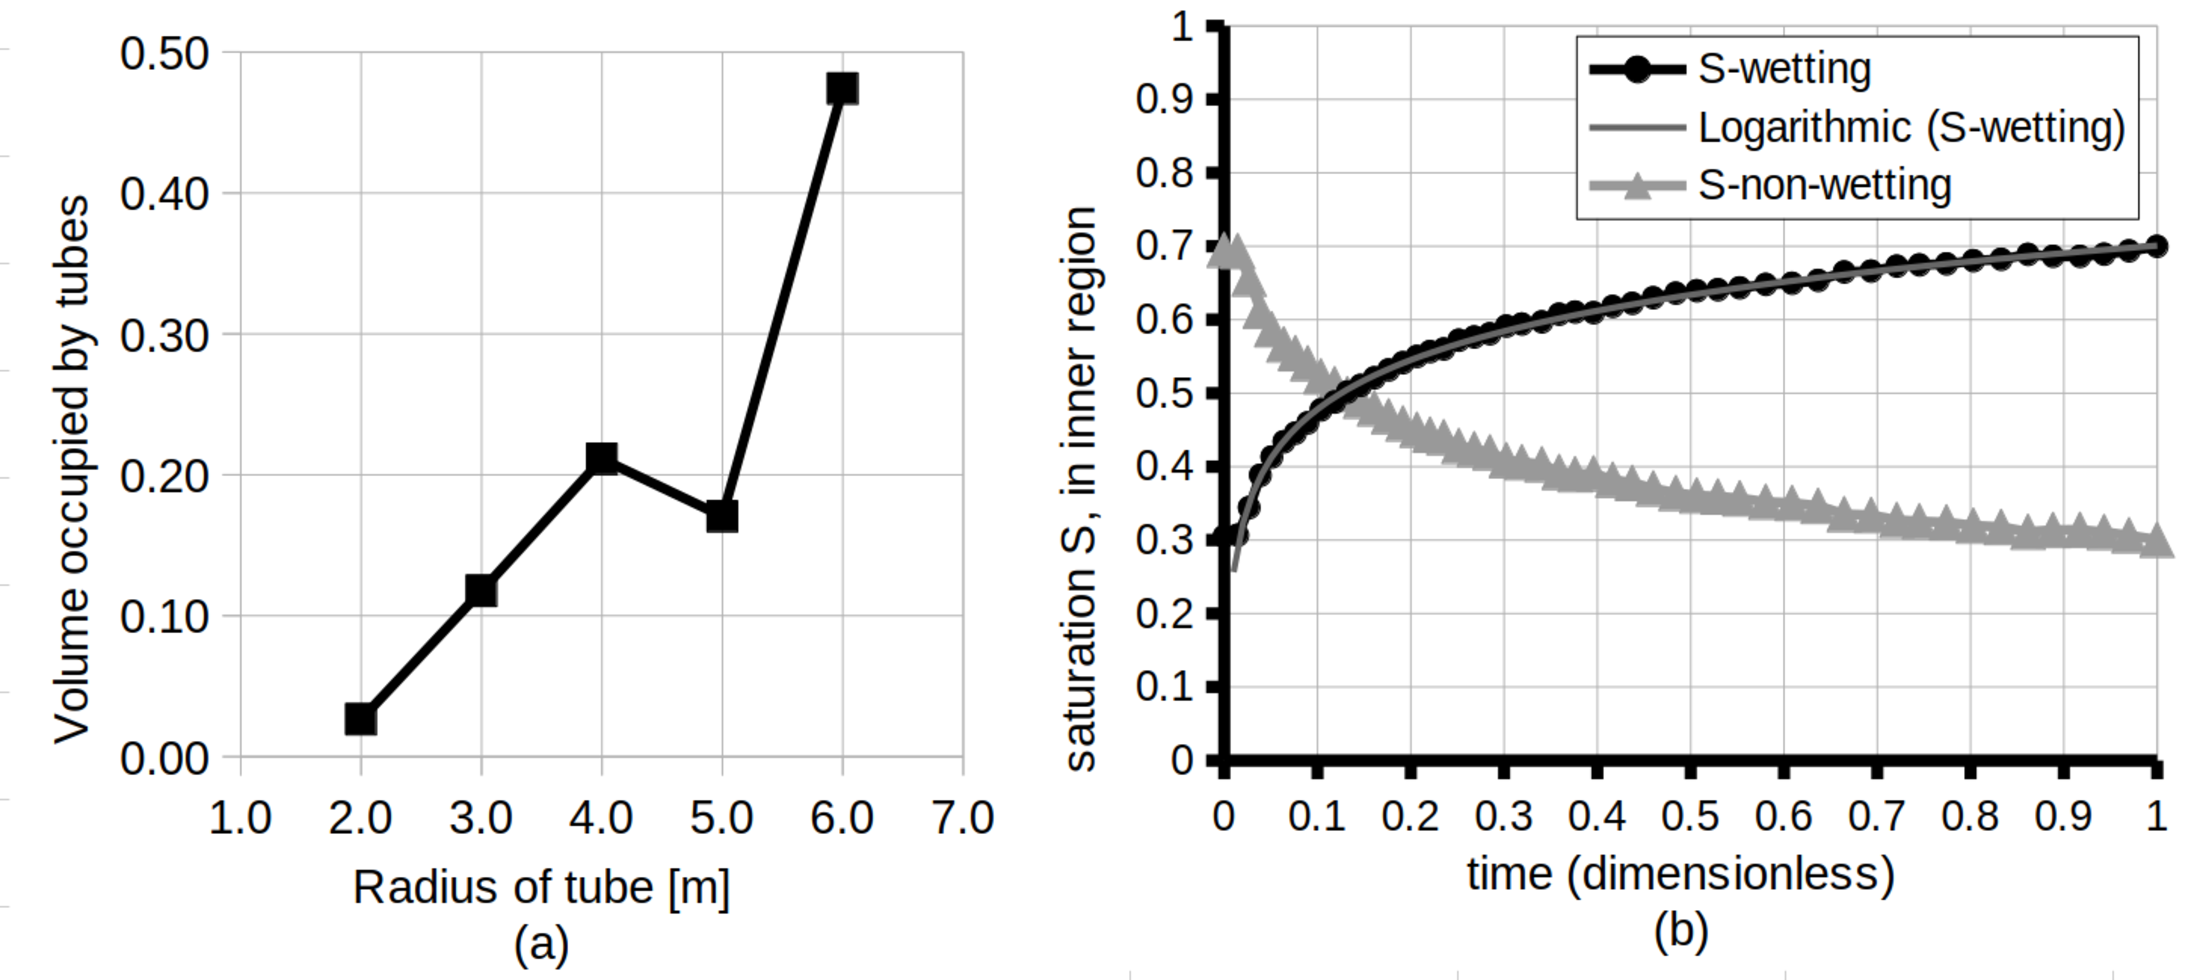
\includegraphics[width=\textwidth]{fig_4_2200x1000}
		\caption{this is a figure-1}
		\label{fig:4}
	\end{figure}
	
	
\subsection{Result of capillary pressure increase}

	\begin{figure}
		\centering
		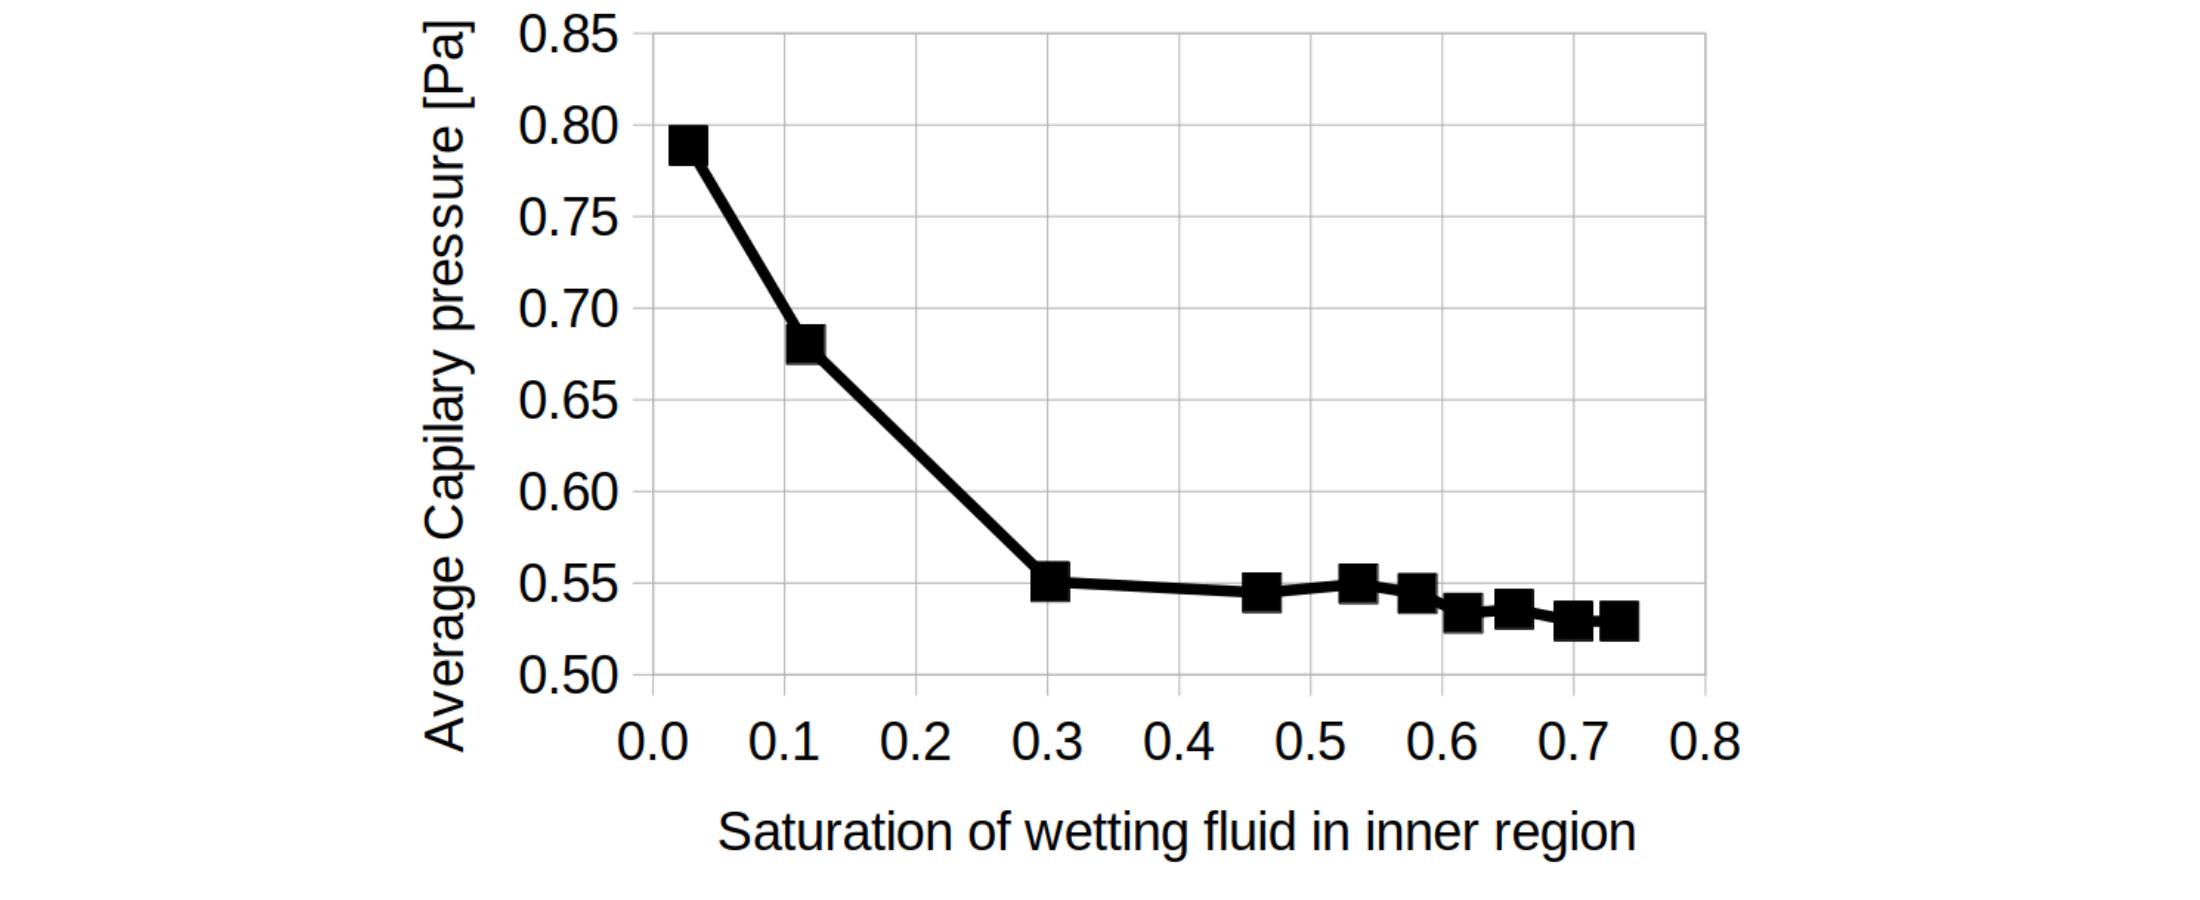
\includegraphics[width=\textwidth]{fig_5_2200x900}
		\caption{this is a figure-1}
		\label{fig:5}
	\end{figure}
	
	Conclusions, the capillary pressure varied depending on its position in the tube. One of the earliest models simulated the flow using a network of electrical resistors \cite{fatt1956network}. 
	
\subsection{Need to read, classify and re distribute info}

	We measured the saturation $S$ vs time $t$ and average capillary pressure $P_c$ vs saturation $S$ only qualitatively. We are interested only in the shape of the curves, therefore time was made dimensionless, and to keep calculations simple the value of radius was in meters. It can be shown that due to the nature of equation \ref{eq:flow-rate-main}, multiplying $R$ by a constant does not change shape of the curve for $S$ vs $t$. In figure \ref{fig:3}, there are $30 \times 30$ order to see the increase of capillary pressure when we decrease the final saturation of wetting fluid in the system, we produced radius distribution 
	
	The final average capillary pressure increased with decreasing the final saturation of wetting (cyan) fluid in the inner region. However since overall less number of meniscus is created in the system is less, we face steps in the experiment where the there is no odd number of meniscus in any tube, and therefore no capillary pressure to continue flow. Therefore for lower than 0.35 initial proportions of blue fluid in the system, the experiment was required to be stopped after a certain number of steps. Since the values of Capillary pressure varied greatly between the 200 steps at which the measurement was recorded, an average of 1000 steps could not be made, therefore further investigation is required to be sure about the increase in capillary pressure.
	
	The algorithm was implemented in C++ 17, compiled using gcc 9.4.0. The computation was performed using processor 11th Gen Intel Core i5-1135G7 @ 2.40GHz operating with Ubuntu 20.04 LTS. The program was not paralleled, hence only one core of the processor was used at a time. The simulation was done for 20,000 steps. Visualization of meniscus configuration and a plot point of saturation $S(t)$ was made for every 200 steps. It took about 1 minute to compile the whole program, and 5 minutes to simulate. If only the radius or initial meniscus configurations are changed, then recompiling is not required. The node located in the center of the system was chosen to have zero pressure. It was observed that changing the node which will have 0 pressure does not change the geometry of the flow.
	
	The plots are not symmetric because small random values $\Delta R / R ~ 10^{-3}$ was introduced to the system. The cyan fluid has invaded from the corners. We decided to plot for $26 x 26$ because a network model of this size can be easily simulated on a personal computer in a short time, and also it satisfies the conditions of gray and cyan fluids having about equal volumes, and the inner radius being 3 times thinner than the outer radius.
		
	The the part of the program slowing down the simulation is the solution of the linear equations using Gaussian-elimination. The process of Gaussian-elimination was not optimized. Hence, if we have $m$ variables, the time complexity for solution is $m^3$. If our network model is of size $n x n$ tubes, then the number of nodes is in the order of $n^2$. Therefore the time to compute grows with the size of the network model in the order of $n^6$. If we doubled the size of the network model, it would take $2^6 = 64$ times longer to perform the same simulation, which is about 5 hours on a personal computer, still reasonable time.
		
	For implementing the algorithm, $double$ is recommended over $float$. $float$ was earlier used to speed up the process by about $2$ times, however the errors grew significantly. The saturation is supposed to remain same due to closed boundaries, but it differed by as much as $10\%$ by the end of the simulation. The error in terms of volume of one of the fluid differing was less than $1\%$ when $double$ was used.
	
	The equilibrium saturation for wetting fluid, $S_{eq} = 0.57$ for the inner region. For different viscosity ratio ${\mu}_1 / {\mu_2}$, the shape of the plot of $S(t)$ does not significantly differ. Changing constants of the experiment such as $\mu, \sigma, l$ simply changes the scale of the $x-axis$. Since the experiment was not calibrated to actual values, we decided to present our result in dimensionless time. It is obtained by simply diving the values on the $x-axis$ by the maximum.
		
	In in $S(t)$ plot of cyan fluid in the inner region. Initially the rate of invasion accelerates at a high rate, then the acceleration slows down, and finally the saturation reaches an equilibrium value which shows only irregular small oscillations. These irregular oscillations is expected to disappear on using a larger network model. They occur to the blocks of wetting fluid remaining in the outer region.
		
	The invasion of cyan fluid occurred from the corners, because in the corners each node is subjected to capillary forces more than from the middle of the edges. And the gray fluid was pushed out from the middle of the edges. The flow stops because of a large number of tubes ending up with 2 menisci. Tubes with two meniscus have a zero net capillary pressure, and cannot initiate flows. 
		
	$S(t)$ approximately shows a logarithmic dependence. It is clear that the relaxation parameter $\xi$ can be applied here the saturation converges to an equilibrium value.
	
	
	astically different initial capillary pressure due to the number of single menisci thinner tubes increased.
			
	The equilibrium saturation for wetting fluid, $S_{eq} = 0.57$ for the inner region. For different viscosity ratio ${\mu}_1 / {\mu_2}$, the shape of the plot of $S(t)$ does not significantly differ. Changing constants of the experiment such as $\mu, \sigma, l$ simply changes the scale of the $x-axis$. Since the experiment was not calibrated to actual values, we decided to present our result in dimensionless time. It is obtained by simply diving the values on the $x-axis$ by the maximum.
			
	In in $S(t)$ plot of cyan fluid in the inner region. Initially the rate of invasion accelerates at a high rate, then the acceleration slows down, and finally the saturation reaches an equilibrium value which shows only irregular small oscillations. These irregular oscillations is expected to disappear on using a larger network model. They occur to the blocks of wetting fluid remaining in the outer region.
	
	The invasion of cyan fluid occurred from the corners, because in the corners each node is subjected to capillary forces more than from the middle of the edges. And the gray fluid was pushed out from the middle of the edges. The flow stops because of a large number of tubes ending up with 2 menisci. Tubes with two meniscus have a zero net capillary pressure, and cannot initiate flows. 
	
	$S(t)$ approximately shows a logarithmic dependence. It is clear that the relaxation parameter $\xi$ can be applied here the saturation converges to an equilibrium value.

	In the previous experiment very slight difference in average capillary pressure is observed when the final saturation of wetting fluid is changed in the inner region. 10 experiments were conducted on 30 x 30 networks with varying radii in the inner region. The initial saturation of the wetting fluid was increased by increasing the proportion of wetting fluid in the inner region. Experiment 2- 10 was done for 10,000 steps. Experiment 1 for 3400 steps and experiment 2 for 1000 steps. This is because in experiment 1 - 2, at some moment complete equilibrium was achieved. There were no tubes with odd number of meniscus remaining in the system, therefore no capillary pressure to drive the flow.
	
	The average capillary pressure at the end is calculated by taking the average of $P_c$ according to equation \ref{eq:average-capillary-pressure} in the last 2000 steps of computation for experiments 2 - 10. Averaging was done to smoothing the effects of the vibrations observed in the capillary pressure. However for experiments 1 – 2, the capillary pressure is not the average of some steps, but for the 1000th step and the 3400th step respectively.
	
	Note that at the step when the experiment was forced to be terminated, capillary pressure cannot be defined. Since the total area in the denominator is zero. Radii of {2, 3, 4, 5} +- 0.01 was used in the inner region. Radius of 6 +- 0.01 was used in the outer region. The outer region was approximately half of the total volume.
	
	Also, it was compulsory to add or substract 0.01 randomness to the radius distributions, because in lower initial saturation of blue fluid in the system, a flow will not start.
	
	Plots of experiment with varying thickness of tubes in the inner region. It can be seen that since it results in total lower energy of the system, it is more frequent to observe that the wetting fluid occupies the thinner tubes than the thicker tubes.
	Experiments conducted, with measurements on the average capillary pressure, initial amount of wetting fluid in the system, final saturation of wetting fluid in the inner region. Note that the final saturation of wetting fluid in the inner region increases with the increase of wetting fluid in the initial conditions.
					
	howing the relative volume occupied by different groups of tubes with different radii. The average capillary pressure is mainly influenced by the thinnest tubes, therefore we see that the final saturation of the wetting fluid in the inner region must be in the order of the volume of the thinnest tube in order to observe significant changes in the average capillary pressure. 
	showing that even with varying radii in the inner region, the saturation change with respect to time remains fairly smooth.
				
	The average capillary pressure rapidly increases with the decrease in final saturation of wetting fluid in the inner region for very low saturations.

	Capillary pressures in tubes of various radii denoted by horizontal straight lines, and plots of capillary pressures for various final saturations of wetting fluid in the inner region. Clearly the average caoillary pressure is situated in between the maximum and minimum horizontal bars.
	Capillary pressure and saturation points for every 200 steps, for high final saturation of wetting fluid in the inner region. We see that the plots tends to end similarly, however has dr
	
\section{Conclusion}
	\begin{enumerate}
		\item The wetting fluid successfully invades the inner region. The wetting fluid in nature prefers to stay in thinner capillaries. Our novel method of distributing different fluids in the nodes, such the wetting fluid first goes into the tube with the thinner radius is valid is therefore valid.
		
		\item We obtained a very smooth plot of $S(t)$, also the fact the saturation tends to an equilibrium value, implies that our network model can be used to simulate other relaxation phenomena, which will help us to better understand the physical meaning of the Kondaurov parameter $\xi$.
		
		\item Our custom definition of calculating the average capillary pressure in a network model must be correct because the capillary pressure increases with decrease of saturation of wetting fluid in the inner region, according to \cite{fatt1956network}.
		
		\item The maximum number of connections a node in our network model can have is 4. Our method of distributing fluids at the node can be easily extended to the more connections per node, hence we plan to extend our model to a 3D case.
		
		\item The fluctuations, once the saturation reaches an equilibrium value is very small. Also the error in terms of fluid lost in a closes system is extremely small. The errors were extremely small because Gaussian-elimination was used to find the pressure in each node. The choice of the method of solving the linear equations defines our speed of computation. We performed our simulation on a network model of a maximum size of $30 \times 30$ tubes, since we wanted each simulation to take a few minutes on a personal computer. We plan to increase the size and study the accuracy of iterative methods.

	\end{enumerate}

\bibliographystyle{plain.bst}
\bibliography{reference}
\end{document}
